\section{An introduction to
Neural Networks}

\subsection{Deep neural networks}
Il termine deep learning si rifà al training di differenti tipi di reti neurali caratterizzate
da diversi layer di neuroni(deep).

Alcuni esempi:
\begin{itemize}
    \item Multi-layer Perceptron with several hidden layers
    \item Convolutional Neural Networks (CNN)
    \item Recurrent Neural Networks (RNN)
    \item Auto-encoder for unsupervised learning
    \item Graph Neural Network (GNN)
    \item Graph Convolutional Network (GCN)
    \item transformers and Attention Models
    \item altri
\end{itemize}

\subsection{Neurone artificiale}

\begin{figure}[H]
    \centering
    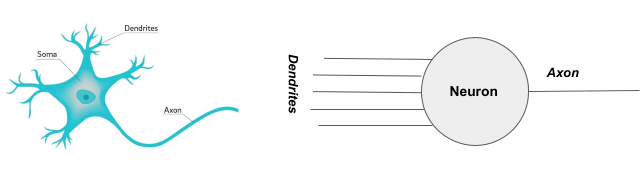
\includegraphics[width=0.5\linewidth]{imgs/neurone-artificale}
    \caption{Neurone artificiale}
    \label{fig:Neurone_artificiale}
\end{figure}

Dove sui dentriti si posizionano le features utili al modello.

Vengono applicati dei pesi e si fa una somma pesata per decidere il risultato.

Manca il bias(intercetta).
\begin{figure}[H]
    \centering
    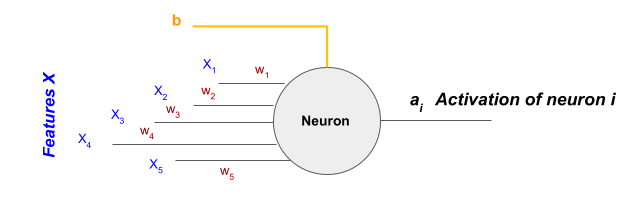
\includegraphics[width=0.5\linewidth]{imgs/neurone}
    \caption{neurone}
    \label{fig:neurone}
\end{figure}

Doev l'attivazione dipende da : $W^{TX+b}$

Fino ad ora molto simile ad una regressione lineare.

Possiamo cambiare la funzione di attivazione!!!

\begin{itemize}
    \item Un neurone artificiale è una funzione che mappa un vettore di features in input
    in uno scalare in output con un vettore di pesi e una funzione
    \item gli input sono i dendriti
    \item il valore scalare dell'output rappresenta l'attivazione del neurone
    \item il neurone riceve gli input pesati, computa l'output secondo la funzione di attivazione
\end{itemize}

\begin{figure}[H]
    \centering
    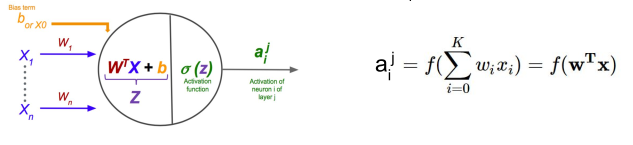
\includegraphics[width=0.8\linewidth]{imgs/neurone2}
    \caption{Funzionamento neurone}
    \label{fig:funzionamento_neurone}
\end{figure}

\subsubsection{Funzione di attivazione}
La funzione f del disegno qui sopra si chiama funzione di attivazione e genera
una relazion non lineare fra input e output.

Ci sono diverse funzioni di attivazione, la più comune è la sigmoide:
\begin{figure}[H]
    \centering
    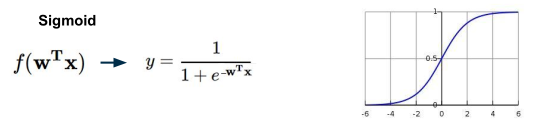
\includegraphics[width=0.7\linewidth]{imgs/sigmoide2}
    \caption{sigmoide}
    \label{fig:sigmoide2}
\end{figure}


\subsubsection{Un layer}
\begin{figure}[H]
    \centering
    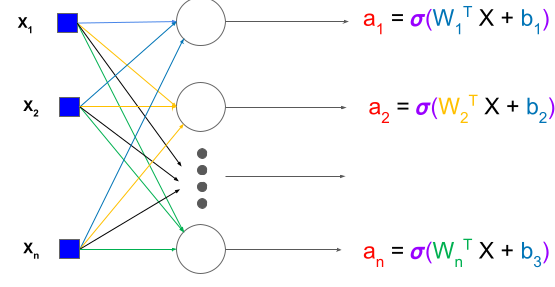
\includegraphics[width=0.7\linewidth]{imgs/layer}
    \caption{layer}
    \label{fig:layer}
\end{figure}


\subsection{Artificial Neural Network(ANN)}
I nodi di uno stattesso layer non counicano tra loro.

Ogni neurone si un layer è collegato a quello del layer successivo e precedente.

\begin{figure}[H]
    \centering
    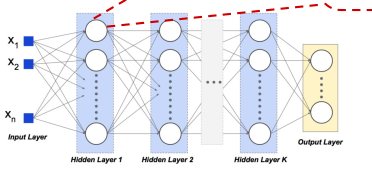
\includegraphics[width=0.6\linewidth]{imgs/ann}
    \caption{ANN}
    \label{fig:ANN}
\end{figure}


Ogni connessione fra neuroni è pesata!!

I pesi sono inizializzati ranodmicamente e l'obbiettivo della rete
durante il training è di imparare i pesi!!

\subsection{Layer di output}
La strutttura di questo laer dipende dal tipo di task.

Il vettore delle Y nel data set deve essere formattato a seconda di questo layer.

\begin{itemize}
    \item regresssione: usimao un neurone per predirre un valore(fuzione di attivazione probabilemte lineare)
    \item classificazione binaria: possimao finire con un neurone che usa una sigmoide(ci sono tanti altri modi)
    \item clssificazione multi classe o multi label: avremmo tanti nodi finali quante le classi(ogni neurone rappresenta una classe)
\end{itemize}


\subsection{Esempi}
\begin{figure}[H]
    \centering
    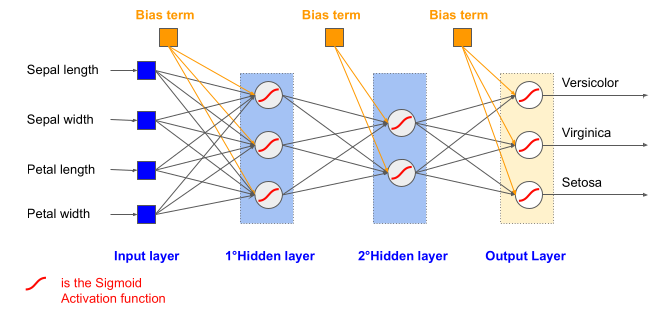
\includegraphics[width=0.8\linewidth]{imgs/iris}
    \caption{iris}
    \label{fig:iris}
\end{figure}
\begin{figure}[H]
    \centering
    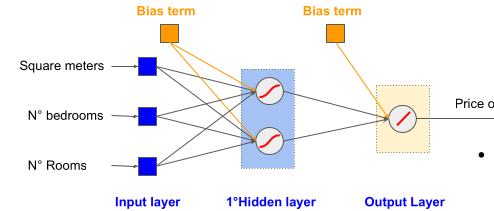
\includegraphics[width=0.8\linewidth]{imgs/case}
    \caption{case}
    \label{fig:case}
\end{figure}

\subsection{Funzioni di attivazione}

\begin{figure}[H]
    \centering
    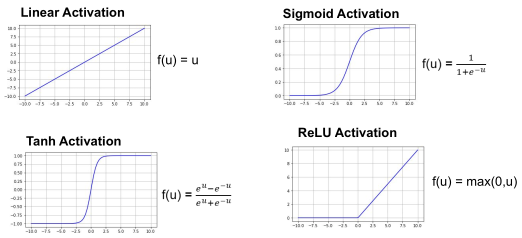
\includegraphics[width=0.8\linewidth]{imgs/funzioni_attivazione}
    \caption{funzioni di attivazione}
    \label{fig:funzioni_attivazione}
\end{figure}

\subsection{Rappresentazione latente}
La rappresentazion latente è quella fra 'ultimo layer nascosto
e il layer di output.

La responsabiltà di fare un task di classificazione o di regressione dipende dal come
viene fatto l'ultimo layer(quello di output).

\subsubsection{Softmax output(solo per la classificazione)}
\begin{figure}[H]
    \centering
    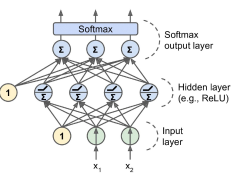
\includegraphics[width=0.5\linewidth]{imgs/softmax}
    \caption{softmax}
    \label{fig:softmax}
\end{figure}

Quando si fa una task di classificazione con multi classe, si può usare un softmax.

Si possono rimpiazzare le indiviuali funzioni del layer che classifica
con una softmax, loutput di ogni neurone (ultimo strato) corrisponde alla
probabilità di appartenere ad una classe.

La softmax è una generalizzazione di unaregressione lineare per supportare
tante classi direttamante senza dover fare una multi classificazione binaria.

La probabilità che un oggetto appartenga alla classe k è:
\begin{equation}
    \vec{p_k} = \sigma(S(X))_k =
    \frac{\exp(s_x(x))}{\sum_{j=1}^{k} \exp(s_j(x))}
\end{equation}

La softmax predice la classe con la maggior probabilità.

\subsection{Reti neurali: ottimizzazione}
\subsubsection{Funzioni di loss}
\begin{figure}[H]
    \centering
    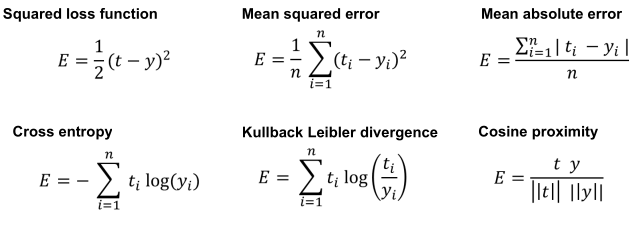
\includegraphics[width=0.8\linewidth]{imgs/funzioni-di-loss}
    \caption{funzioni di loss}
    \label{fig:funzioni_di_loss}
\end{figure}

\begin{itemize}
    \item task di regressione
    \begin{itemize}
        \item mean squared error loss
        \item mean absolute error loss
    \end{itemize}
    \item task di classificazione binaria
    \begin{itemize}
        \item binary cross-entropy
    \end{itemize}
    \item task classificazione multi-classe
    \begin{itemize}
        \item multi-class cross-entropy loss
        \item Kullback Leibler Divergence Loss
    \end{itemize}
\end{itemize}


\subsection{Allenanod un ANN: algortimi di backpropagation}

\begin{enumerate}
    \item inizializzo un ANN con pesi random
    \item propago ogni esempio nella rete dal input layer fino al layer di
    output e ottengo una predizione
    \item poi calcolo l'errore della predizione(differenza tra vero e predetto)
    \item misuro l'errore e provo a risurre l'errore aggiornando i pesi,
    propago l'errore indietro fino all'input
\end{enumerate}

\subsubsection{Backpropagation}
\begin{itemize}
    \item l'errore viene propagato fino all'input per aggiornare i pesi
    \item per sapere come aggioranre i pesi, dobbiamo fare il gradiente
    \item quindi si fa il gradiente per ogni layer partendo dall'output fino ad arrivare
    all'input
\end{itemize}

Si fa una discesa del gradiente per ridurre l'errore.

Il nuovo peso assume questo valore:
\begin{figure}[H]
    \centering
    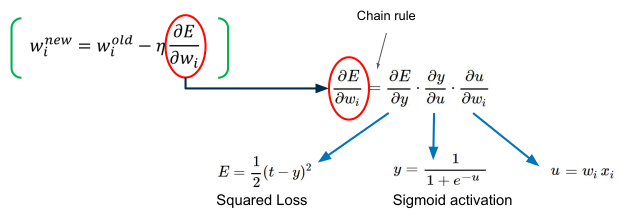
\includegraphics[width=0.8\linewidth]{imgs/discesa-del-gradiente-ann}
    \caption{discesa del gradiente ANN}
    \label{fig:discesa_del_gradiente_ANN}
\end{figure}
\begin{figure}[H]
    \centering
    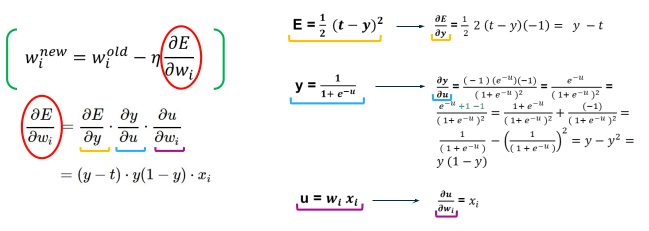
\includegraphics[width=0.8\linewidth]{imgs/discesa-del-gradiente-ann2}
    \caption{discesa del gradiente ANN parte 2}
    \label{fig:discesa_del_gradiente_ANN2}
\end{figure}

Ricordo che $\eta$ è la lunghezzaa del passo della discesa del gradiente(velocita di apprendimento).

Poi si aggiornano i pesi e si continua fino ad un risoltato soddisfacente.

\subsection{Hyper parameters}
Sono i parametri che definiscono la struttura della rete neurale e i paramtri
che determinano come la rete verrà allenata:
\begin{itemize}
    \item numero di neuroni
    \item numero di layer
    \item lernign rate
    \item batch size
    \item numero si epochs
    \item altri
\end{itemize}

\subsubsection{Learnig rate}
\begin{figure}[H]
    \centering
    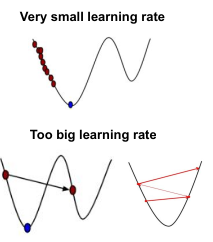
\includegraphics[width=0.3\linewidth]{imgs/learning-rate}
    \caption{learning rate}
    \label{fig:learning_rate}
\end{figure}

Bisogna usare un learning rate approppriato perchè se troppo piccolo(fig: 1)
si rischia di impiegarci troppo tempo, se invece si usa un learnign rate troppo
grande, si rischia di non trovare il minimo e "saltare" oltre(fig: 2).

\subsubsection{Numero di epochs}
Il numero di epochs è il numero di volte che l'intero training set viene mostrato
alla rete neurale durante l'allenamento.

\subsubsection{Batch size}
Il numero di campioni fattti vedere all rete prima della discesa del gradiente.

\subsection{Validation set}
Stessa funzione del test set ma viene fatto vedere durante il training
per effetuare un fine tuning della rete.

Permette di avere un feedback per migliorare il sistema.

\subsection{Early stopping}


\begin{figure}[H]
    \centering
    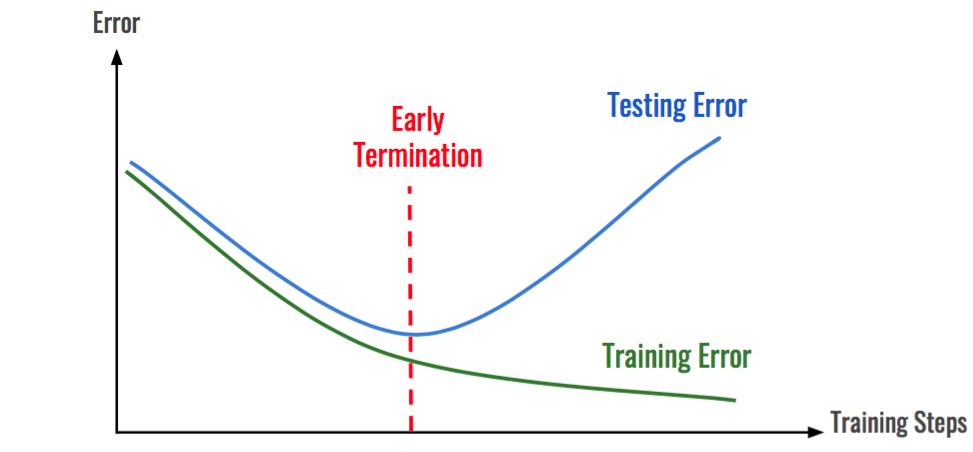
\includegraphics[width=0.5\linewidth]{imgs/early-stopping}
    \caption{early stopping}
    \label{fig:early_stopping}
\end{figure}

È una forma di regularizzation usata per evitare l'overfitting con metodi interattivi
come la discesa del gradiente.

Si ferma quando nota che la forbice che dell'errore si allarga.

Si può definire un parametro di pazienza, accettiamo che l'errore possa essere
più alto del valore precedente per un numer odi volte, dopo di che
il sistema si ferma, vengon usati i pesi delle iterazioni precedenti.

\subsection{Dropout}
È un'altra forma di regularizzation per le reti neurali, durante il training,
randomicamente alcuni nodi vengon esclusi per evitare l'overfitting.

\begin{figure}[H]
    \centering
    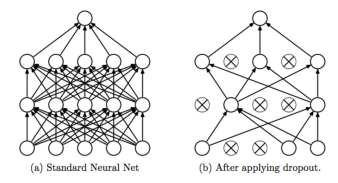
\includegraphics[width=0.3\linewidth]{imgs/drop-out}
    \caption{dropout}
    \label{fig:dropout}
\end{figure}


\subsection{Scegliere la funzione di loss per le ottimizzazioni}
Per minimizzare l'errore non abbiamo solo la discesa del gradiente(GD) o
la discesa stocastica del gradiente(SGD), altre ottimizzazioni basate sul gradiente
sono :
\begin{itemize}
    \item RMSprop
    \item Adam
\end{itemize}

È importante capire profondamente il problema per caapire cosa scegliere per ottimizzare.

\subsection{Keras}
Keras è una libreria open-source che fornisce strumenti per le ANN(artificial
neural network).

Keras funziona come interfaccia per TensorFlow.





































